\documentclass[letterpaper,11pt]{article}
\pdfoutput=1 % if you are submitting a pdflatex (i.e. if you have
             % images in pdf, png or jpg format)

\usepackage{jheppub} 
%\usepackage[T1]{fontenc} % if needed
%\usepackage[latin1]{inputenc}
\usepackage{graphicx}
\usepackage{amsmath}
\usepackage{amsfonts}
\usepackage{slashed}
\usepackage{amssymb}
\usepackage{hyperref}
	\hypersetup{colorlinks=true, linkcolor=blue, citecolor=red, urlcolor=cyan, linktoc=page}
%\usepackage{cite}
\usepackage{xfrac}
\usepackage{empheq}
\usepackage{caption, subcaption}

\newcommand{\p}{\partial}
\newcommand{\oi}{\omega_i}
\newcommand{\oj}{\omega_j}
\newcommand{\ok}{\omega_k}
\newcommand{\ol}{\omega_l}
\newcommand{\mc}{\mathcal}

%%%%%%%%%%%%%%%%%%%%%%%%%%%%%%%%%%%%%%%%%
%%%%%%%%%%%%%%%%%%%%%%%%%%%%%%%%%%%%%%%%%

\title{Two-Time Formalism in AdS$_4$}

\author[a]{Brad Cownden,}

\author[b]{Nils Deppe,}

\author[a,c]{Andrew R.~Frey}

\affiliation[a]{Department of Physics \& Astronomy\\ University of Manitoba,
Winnipeg, Manitoba R3T 2N2, Canada}

\affiliation[b]{Cornell Centre for Astrophysics and Planetary Science\\ Cornell University, Ithaca, New York 14853, USA}

\emailAdd{cowndenb@myumanitoba.ca}
\emailAdd{nd357@cornell.edu}
\emailAdd{a.frey@uwinnipeg.ca}

\abstract{We construct a family of perturbative solutions for massless scalar fields in AdS$_4$ using the \emph{Two-Time Formalism} (TTF) to high eigenmode numbers. We furthermore investigate the validity of \emph{quasi-periodic} (QP) solutions with high $j_{max}$ values and examine their stability to perturbations. Finally, check that TTF and QP solutions continue to satisfy the Einstein equation at times greater than $t \sim \epsilon^{-2}$ and compare these results to the full numerical solutions at low amplitude.}

\keywords{AdS/CFT}

%%%%%%%%%%%%%%%%%%%%%%%%%%%%%%%%%%%%%%%%%
%%%%%%%%%%%%%%%%%%%%%%%%%%%%%%%%%%%%%%%%%

\begin{document}
\maketitle
\flushbottom

\section{Introduction}

%%%%%%%%%%%%%%%%%%%%%%%%%%%%%%%%%%%%%%%%%

\section{Two-Time Formalism}

Consider a spherically-symmetric, asymptotically AdS$_{d+1}$ spacetime compactified on a circle of radius $x$, whose metric is given by
\begin{align}
ds^2 = \frac{\ell^2}{\cos^2(x\ell)} \left( Ae^{-2\delta} dt^2 + A^{-1}dx^2 + \sin^2(x\ell) d\Omega^{d-1}\right) \, ,
\end{align}
where the radius is $x \in [0,\pi/2)$, $-\infty < t < \infty$, and $a, b \in \{0,\ldots,d\}$. Taking $\ell = 1$, a scalar field $\phi(t,x)$ with mass $\mu$ is subject to the following Einstein and Klein-Gordon equations:
\begin{align}
G_{ab} + \Lambda g_{ab} &= 8\pi \left( \nabla_a \phi \nabla_b \phi - \frac{1}{2} g_{ab} \big( (\nabla \phi)^2 + \mu^2 \phi^2 \big) \right) \\
\mu^2 \phi &= \frac{1}{\sqrt{-g}} \p_a \sqrt{-g} \, g^{ab} \p_b \phi \, .
\end{align}

The linearized system allows for the field to be written in terms of eigenfunctions of the operator $L$ given by
\begin{align}
\label{linized}
\p_t^2 \phi = \left( \frac{(d-1)}{\sin(x) \cos(x)} \p_x + \p^2_x - \frac{\mu^2}{\cos^2(x)}\right) \phi = - L \phi \, .
\end{align}
The solutions to \eqref{linized} are the normalized Jacobi polynomials,
\begin{align}
\label{eigens}
e_j(x) = k_j \cos^{\lambda_{\pm}}(x) P^{(\frac{d}{2} - 1, -\frac{d}{2} + \lambda_{\pm})}_j (\cos(2x)) \, ,
\end{align}
whose eigenvalues are $\omega_j = \lambda_{\pm} + 2j$, with $\lambda_\pm$ given by $\lambda_{\pm} = (d \pm \sqrt{d^2 + 4\mu^2})/2$.

The Two-Time Formalism (TTF) describes the solution to \label{linized} in terms of slowly-modulating amplitude and phase variables, $A_j$ and $B_j$, that are functions of the slow time $\tau = \epsilon^2 t$,
\begin{align}
\label{phi ttf}
\phi(t,x) = \epsilon \sum_{j=0}^\infty A_j (\epsilon^2 t) e_j(x) \cos \left(\omega_j t + B_j(\epsilon^2 t) \right).
\end{align}
The next non-trivial order in the equations of motion include gravitational self-interactions of the scalar field, and provides source terms for $A_j$ and $B_j$. Following the time-averaging procedure of \cite{1407.6273} -- and using the resonance condition $\oi + \oj = \ok + \ol$ to eliminate one of the indices -- the $l^{th}$ amplitude and phase are given by
\begin{align}
\label{RN1}
-\frac{2\omega_l}{\epsilon^2} \frac{d A_l}{d t} &= \stackrel{l \leq i + j}{\sum_{i \neq l} \sum_{j \neq l}} S_{ij (i + j -l) l} A_i A_j A_{i + j - l} \sin \left( B_l + B_{i+j-l} - B_i - B_j \right) , \\
\label{RN2}
- \frac{2 \omega_l A_l}{\epsilon^2} \frac{d B_l}{dt} &= T_l A_l^3 + \sum_{i \neq l} R_{i l} A^2_i A_l  \nonumber \\
& \qquad + \stackrel{l \leq i + j}{\sum_{i \neq l} \sum_{j \neq l}} S_{ij (i + j -l) l} A_i A_j A_{i + j - l} \cos \left( B_l + B_{i+j-l} - B_i - B_j \right) \, .
\end{align}
The coefficients $T, R, S$ are calculated directly from integrals over the product of eigenmodes and contain some useful symmetry properties: the integrals vanish except with the resonance condition $\omega_i + \omega_j = \omega_l$ is met. 

Computationally, we find it more convenient to write $T, R, S$ in terms of axillary coefficients with greater symmetry properties (as shown in \cite{1508.04943})\footnote{The final terms in \eqref{T calc} and \eqref{R calc} differ from \cite{1508.04943} since we have chosen to work in the boundary gauge.}
\begin{align}
\label{T calc}
T_l &= \frac{1}{2} \ol^2 X_{llll} + \frac{3}{2} Y_{llll} + 2\omega_l^4 W_{llll} + 2\omega_l^2 W^*_{llll} - \omega_l^2 (A_{ll} + \omega_l^2 V_{ll} ) \\
\label{R calc}
R_{il} &=\frac{1}{2} \left(\frac{\oi^2 + \ol^2}{\ol^2 - \oi^2}\right) (\omega_l^2 X_{illi} - \omega_i^2 X_{liil}) + 2\left(\frac{\ol^2 Y_{ilil} - \oi^2 Y_{lili}}{\ol^2 - \oi^2} \right) \nonumber \\
&+ \left(\frac{\oi^2 \ol^2}{\ol^2 - \oi^2}\right) (X_{illi} - X_{lili}) + \frac{1}{2} (Y_{iill} + Y_{llii}) + \oi^2 \ol^2 (W_{llii} + W_{iill}) \nonumber \\
&+ \oi^2 W^*_{llii} + \ol^2 W^*_{iill} - \ol^2 (A_{ii} + \omega_i^2 V_{ii} ) \\
\label{S calc}
S_{ijkl} &= -\frac{1}{4} \left( \frac{1}{\omega_i + \omega_j} + \frac{1}{\omega_i - \omega_k} + \frac{1}{\omega_j - \omega_k} \right) (\omega_i \omega_j \omega_k X_{lijk} - \omega_l Y_{iljk}) \nonumber \\
& - \frac{1}{4} \left( \frac{1}{\omega_i + \omega_j} +\frac{1}{\omega_i - \omega_k} - \frac{1}{\omega_j - \omega_k} \right) (\oj \ok \ol X_{ijkl} - \oi Y_{jikl} ) \nonumber \\
& -\frac{1}{4} \left( \frac{1}{\oi + \oj} - \frac{1}{\oi - \ok} + \frac{1}{\oj -\ok} \right) (\oi \ok \ol X_{jikl} - \oj Y_{ijkl} ) \nonumber \\
& -\frac{1}{4} \left( \frac{1}{\oi + \oj} - \frac{1}{\oi - \ok} - \frac{1}{\oj - \ok} \right) (\oi \oj \ol X_{kijl} - \ok Y_{ikjl}) \, ,
\end{align}
where the integrals $X_{ijkl}$, $Y_{ijkl}$, $W_{ijkl}$, $W^*_{ijkl}$, $A_{ij}$, and $V_{ij}$ are products of the eigenfunctions in \eqref{eigens} and their derivatives. Explicitly, they are
\begin{align}
\label{X int}
X_{ijkl} &= \int^{\pi/2}_0 dx \, e'_i(x) e_j(x) e_k(x) e_l(x) \sin(x) \cos(x) \left( \tan(x) \right)^{d-1} \\
\label{Y int}
Y_{ijkl} &= \int^{\pi/2}_0 dx \, e'_i(x) e_j(x) e'_k(x) e'_l(x) \sin(x) \cos(x) \left( \tan(x) \right)^{d-1} \\
\label{W int}
W_{ijkl} &= \int^{\pi/2}_0 dx \, e_i(x) e_j(x) \sin(x) \cos(x) \int^x_0 dy \, e_k(y) e_l(y) \left( \tan(y) \right)^{d-1} \\
\label{W* int}
W^*_{ijkl} &= \int^{\pi/2}_0 dx \, e'_i(x) e'_j(x) \sin(x) \cos(x) \int^x_0 dy \, e_k(y) e_l(y) \left( \tan(y) \right)^{d-1} \\
\label{A int}
A_{ij} &= \int^{\pi/2}_0 dx \, e'_i(x) e'_j(x) \sin(x) \cos(x) \\
\label{V int}
V_{ij} &= \int^{\pi/2}_0 dx \, e_i(x) e_j(x) \sin(x) \cos(x) \, .
\end{align}

Using a complex amplitude of the form $\mc A_j(\tau) = A_j \exp (-i B_j )$ in \eqref{phi ttf} allows us to combine equations \eqref{RN1} and \eqref{RN2} into a single TTF equation:
\begin{align}
\label{ttf eqn}
-2i \ol \frac{\mc A_l}{d \tau} = T_l |\mc A_l|^2 \mc A_l + \sum_{i \neq l} R_{il} |\mc A_i|^2 \mc A_l + \stackrel{l \leq i+j}{\sum_{i \neq l} \sum_{j \neq l}} S_{ij(i+j-l)l} \mc A_i \mc A_j \bar{\mc A}_{i+j-l} \, .
\end{align}

%%%%%%%%%%%%%%%%%%%%%%%%%%%%%%%%%%%%%%%%%

\section{Quasi-periodic Solutions}
The stability of the solutions to \eqref{ttf eqn} can be examined using a \emph{quasi-periodic} (QP) ansatz for the complex amplitude,
\begin{align}
\mc A_j = \alpha_j e^{i \beta_j \tau} \, ,
\end{align}
where $\alpha_j, \beta_j \in \mathbb{R}$. The time dependence in \eqref{ttf eqn} is removed via the condition $\beta_j = \beta_0 + j(\beta_1~-~\beta_0)$, leaving $\beta_0$ and $\beta_1$ as unknown parameters. Considering modes of \eqref{phi ttf} up to some $j_{max}$, the QP ansatz results in a set of $j_{max} + 1$ algebraic equations for $j_{max} + 3$ unknowns
\begin{align}
\label{qp eqn}
2 \omega_l \alpha_l \beta_l = T_l \alpha_l^3 + \sum_{i \neq l} R_{il} \alpha_i^2 \alpha_l + \stackrel{l \leq i + j}{\sum_{i \neq l} \sum_{j \neq l}} S_{ij(i+j-l)l} \alpha_i \alpha_j \alpha_{i+j-l} \, .
\end{align}
As shown in \cite{1507.08261}, the TTF is invariant under a $U(1)$ transformation that leads to the conserved quantities
\begin{align}
\label{qp cons}
E = 4\sum_j \omega^2_j \alpha_j^2 \qquad \text{and} \qquad N= 4 \sum_j \omega_j \alpha_j^2 \, .
\end{align}
These definitions allow for two of the free parameters to be fixed. Families of solutions can be examined by fixing $\alpha_0 = 1$ and sampling a range of $\alpha_1$ values in the range $\alpha_1 \ll \alpha_0$. The families of solutions can be distinguished by their ``temperature'', or energy per particle number $T=E/N$. 

The question of edge effects in determining the stability of a particular solution is important to investigate. For instance, if a particular solution to \eqref{qp eqn} is found for some $\alpha_1$ when $j_{max} = 50$, does this continue to be a solution when we consider more modes, say $j_{max} = 250$? By following the methods outlined in appendix~\ref{app: seeding}, we are able to start with a low $j_{max}$ solution and incrementally increase the number of modes being considered up to several hundred. This method was found to be more successful, given the optimization algorithms being used, than other seeding methods.

As an example, consider solutions to \eqref{qp eqn} with the conditions $\alpha_0 = 1.0$ (since all QP solutions are defined up to an overall scale, $\alpha_0 = 1.0$ is taken to always be true) and $\alpha_1 = 0.2$, which corresponds to an initial temperature of $T_0 \simeq 3.146$. In figure~\ref{fig: a0.2solns}, we see that an initial solution when $j_{max}=50$ persists as $j_{max}$ is increased to $200$. However, some solutions -- such as those shown in figure~\ref{fig: a0.36solns} -- fail as $j_{max}$ is increased. 

\begin{figure}[h]
	\centering
	\begin{subfigure}[t]{0.45\textwidth}
		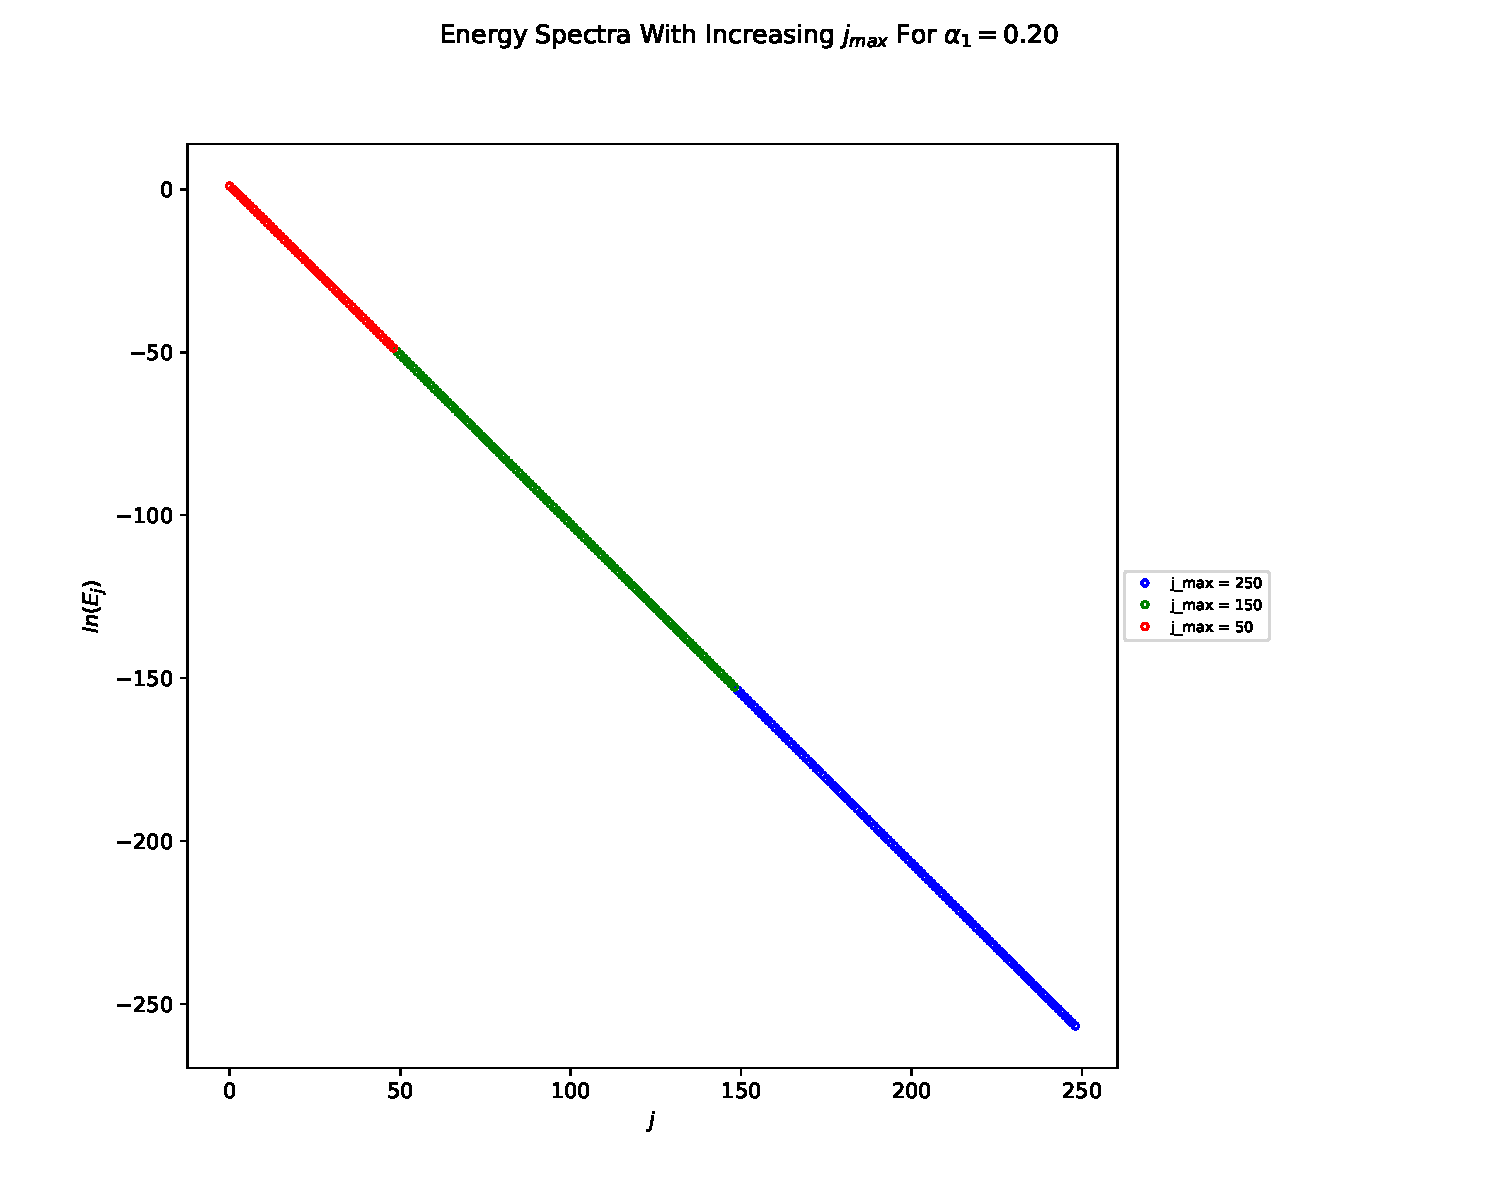
\includegraphics[width=\textwidth]{a0_2overlay}
		\caption{An overlay of QP solutions with $\alpha_1 = 0.2$, corresponding to $T_0 \simeq 3.146$. As $j_{max}$ is increased, the solution continues to be valid; therefore, it is not an artifact of the choice of truncation value of $j_{max}$.}
		\label{fig: a0.2solns}
	\end{subfigure}
	\:
	\begin{subfigure}[t]{0.45\textwidth}
		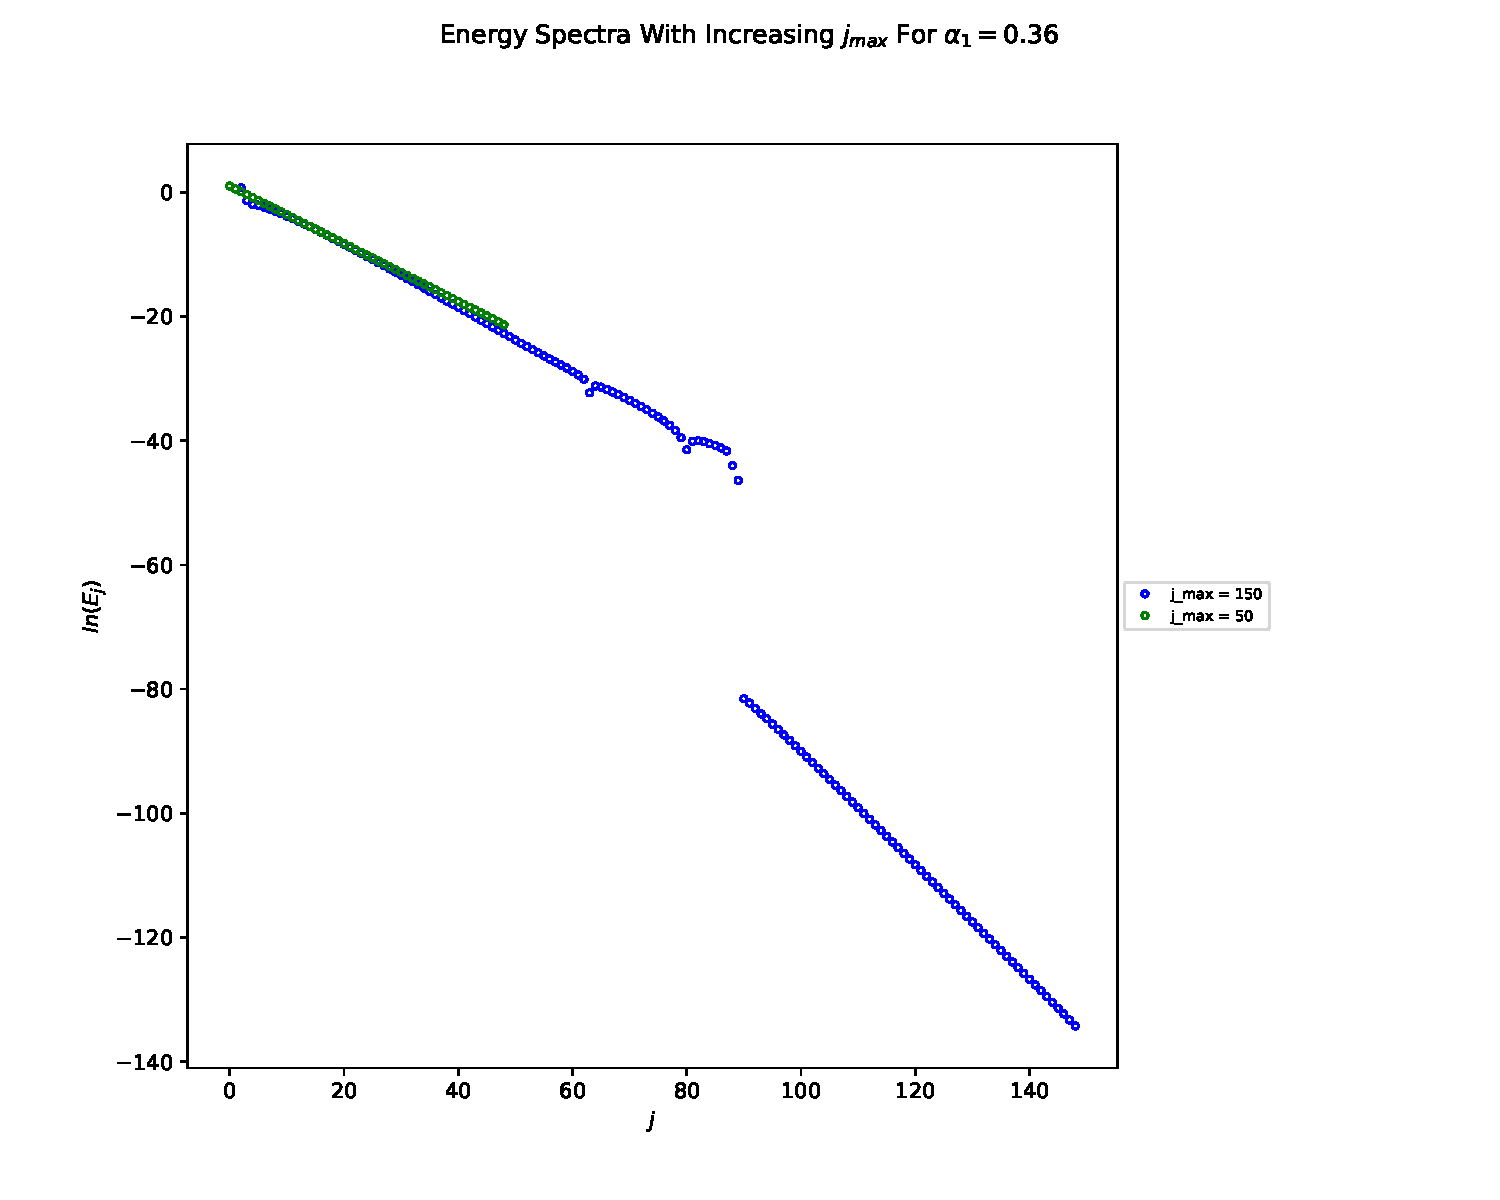
\includegraphics[width=\textwidth]{a0_36overlay}
		\caption{While a solution does exist for $\alpha_1 = 0.36$ ($T_0 \simeq 3.623$) when $j_{max}=50$, we see that the solution is no longer smooth when $j_{max}=150$ and in fact does not exist when $j_{max}=250$.}
		\label{fig: a0.36solns}
	\end{subfigure}
	\caption{Overlays of two QP solutions that are valid for small $j_{max}$, but are not necessarily valid with increasing $j_{max}$.}
\end{figure}

\subsection{High Temperature Perturbations}
In \cite{1507.08261}, additional QP solutions can be found by perturbing existing solutions. The addition of some energy $\delta E$ corresponds to the changes $\alpha_j \to \alpha_j + u_j$ and $\beta_j \to \beta_j + \theta_1 + \omega_j \theta_2$. The perturbed quantities are given by the system of \emph{linear} equations
\begin{align}
\label{HT1}
\delta E &= 4 \sum_j \omega^2_j \alpha_j u_j \\
\label{HT2}
\delta N &= 4 \sum_j \oj \alpha_j u_j = 0 \\
\label{HT3}
0 &= \ol \left( \alpha_l (\theta_1 + \ol \theta_2) +\beta_l u_l \right) + 6T_l \alpha_l^2 u_l + 2 \sum_{i \neq l} R_{il} (\alpha_i^2 u_l + 2 \alpha_i \alpha_l u_l ) \nonumber \\
& + 2 \stackrel{l \leq i + j}{\sum_{i \neq l} \sum_{j \neq l}} S_{ij(i+j-l)l} \left[ u_i \alpha_j \alpha_{i+j-l} + u_j \alpha_i \alpha_{i+j-l} + \alpha_i \alpha_j u_{i+j-l} \right].
\end{align}
Therefore, by solving \eqref{HT1}-\eqref{HT3} for $\{ u_j, \theta_1, \theta_2 \}$, the existing QP solution can be updated and the process can be repeated. 

For a standard QP solution with $\alpha_0 = 1$ (this is value is kept fixed by rescaling the values of $\alpha_j$ when required) and $\alpha_1 = 0.2$, the solution is initially characterized by the temperature $T_0 = 3.146$. By applying the high temperature perturbation method described above, we are able to increase the temperature of the solution. However, this process must be examined with some scrutiny; applying repeated perturbations to a known solution does not guarantee the final result remains a valid solution. To investigate this further, we have implemented a solver that projects back down to the QP solution plane after either a set number of perturbations, or after every perturbation. When a perturbed solution can no longer be projected back to the QP plane, we have perturbed too far and the state no longer represents a quasi-periodic TTF solution. An example of this kind of verified spectrum is shown in figure~\ref{fig: verified}.

\begin{figure}[h]
\centering
  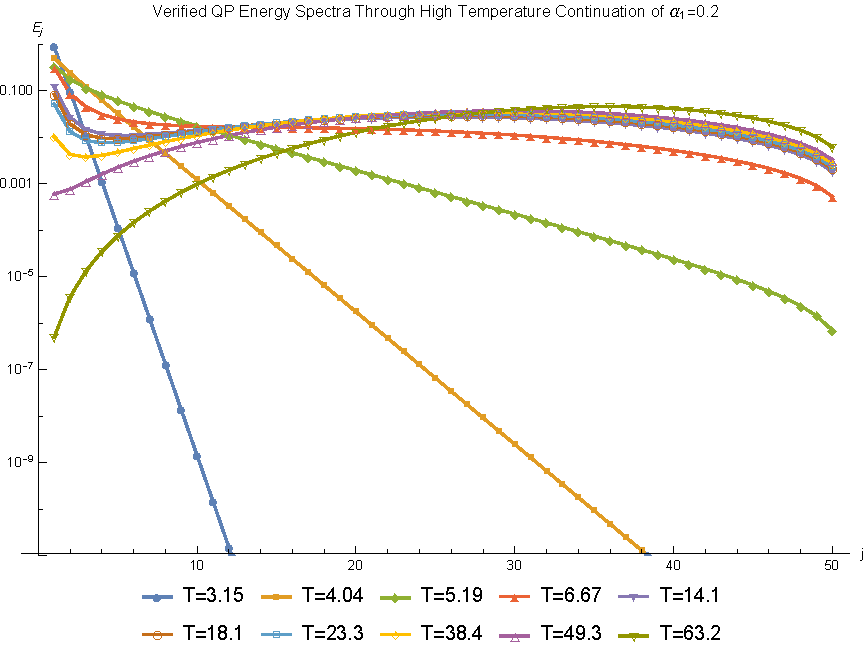
\includegraphics[scale=0.75]{a20HighTE} 
  \caption{Verified energy spectra for $\alpha_1 = 0.2$. These profiles include only those solutions that were able to be projected back to the QP solution plane.}
  \label{fig: verified}
\end{figure}






%%%%%%%%%%%%%%%%%%%%%%%%%%%%%%%%%%%%%%%%%
%%%%%%%%%%%%%%%%%%%%%%%%%%%%%%%%%%%%%%%%%

\acknowledgments{The work of A.~F.~and B.~C.~ has been supported by NSERC and through a Westgrid allocation with Compute Canada.}

%%%%%%%%%%%%%%%%%%%%%%%%%%%%%%%%%%%%%%%%%
%%%%%%%%%%%%%%%%%%%%%%%%%%%%%%%%%%%%%%%%%

\appendix

\section{Seeding Methods For Non-Linear Solvers}
\label{app: seeding}
While it was originally proposed by \cite{1507.08261} that the appropriate seed value for nonlinear solvers be given by the exponential energy spectrum ($j > 1$)
\begin{align}
\label{old seed}
\alpha_j \sim \frac{3 e^{-\mu j}}{2j + 3}
\end{align}
in AdS$_4$, where $\mu = \ln (3 / 5 \alpha_1 )$. Although this profile was sufficient for low $j_{max}$ solutions, above $j_{max} \gtrsim 150$, \eqref{old seed} no longer provided an adequate starting guess. To overcome this problem, exponential fitting was applied to the tail values of a known QP solution with lower $j_{max}$. Using this exponential fit, the data was extrapolated to a higher $j_{max}$. Care was taken to avoid edge effects when choosing the points that constituted the tail of the data. It was found that the modes $[ j_{max} - 30, j_{max} - 10]$ remained unaffected by edge effects and provided more accurate seed values for $j_{max} + 25$ solutions. See figure~\ref{fig: tail fitting} for a comparison of seed values generated by tail fitting to actual QP solutions. The solutions found using this method of seeding versus those found from the seeding given in \eqref{old seed} had relative differences on the order of $10^{-14}$ (see figure~\ref{fig: seedvsunseed}).

\begin{figure}[h]
\centering
  	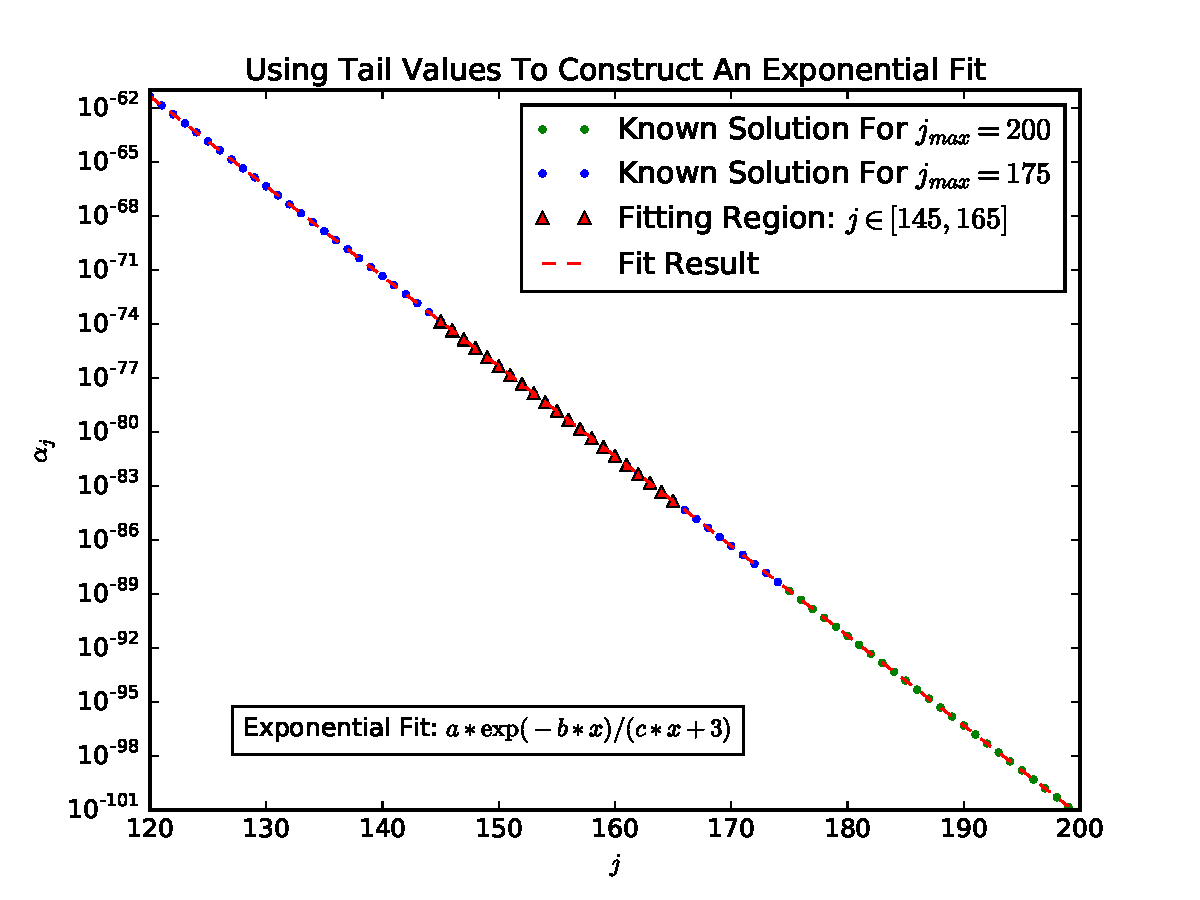
\includegraphics[scale=0.5]{TailFitPlot}
  	\caption{Fitting the tail of the $j_{max} = 175$ spectrum to construct a seed for $j_{max} = 200$ at fixed $\alpha_1$. Also included is actual QP spectrum for $j_{max} = 200$.}
  	\label{fig: tail fitting}
\end{figure}
\begin{figure}[h]
  	\centering
	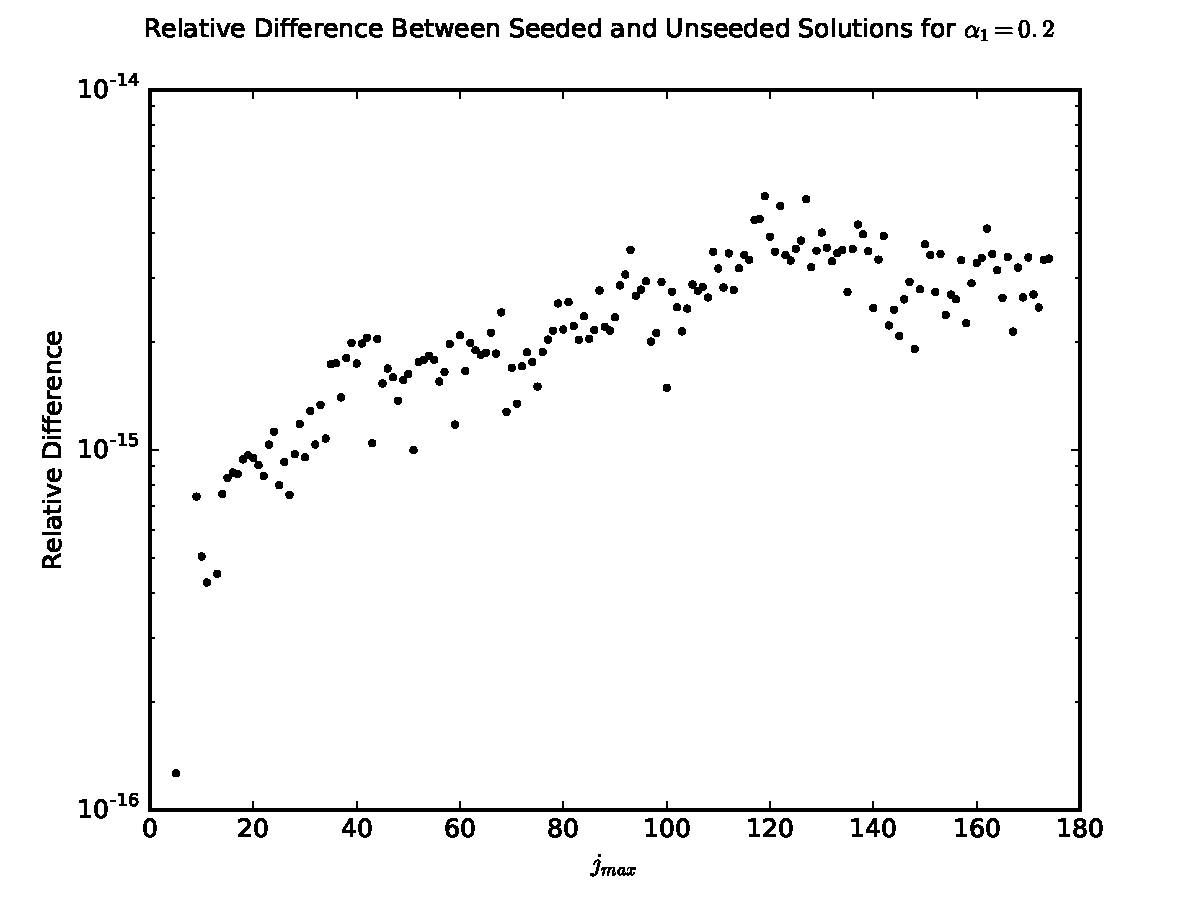
\includegraphics[scale=0.5]{SeedvsUnseed}
	\caption{Relative difference between QP solutions found using tail fitting and those from the exponential profile~\eqref{old seed}}
	\label{fig: seedvsunseed}
\end{figure}

%%%%%%%%%%%%%%%%%%%%%%%%%%%%%%%%%%%%%%%%%
%%%%%%%%%%%%%%%%%%%%%%%%%%%%%%%%%%%%%%%%%

\bibliographystyle{JHEP}
\bibliography{TTFbib}

%%%%%%%%%%%%%%%%%%%%%%%%%%%%%%%%%%%%%%%%%
%%%%%%%%%%%%%%%%%%%%%%%%%%%%%%%%%%%%%%%%%

\end{document}

%%%%%%%%%%%%%%%%%%%%%%%%%%%%%%%%%%%%%%%%%
%%%%%%%%%%%%%%%%%%%%%%%%%%%%%%%%%%%%%%%%%



